\section{Preliminary Models}
\subsection{Daimler Models}

\subsubsection*{Introduction}

As previously described in D1.2 and the DoW, the basic settings of the DAIMLER's use-case are as follows. Let us suppose we are driving our car, which will be referred as the EGO vehicle, in a highway. This EGO vehicle is equipped with a video camera, radar and some on-board sensors.  Using the data provided by these sensors, the problem consists in the early recognition a maneuver either of the EGO or another relevant car in the traffic scene. In total, the system is expected to recognized the following set of of maneuvers (a visual description of them is given below in Figure \ref{Figure:DaimlerManeuvers}):
\begin{enumerate}

\item \textbf{Object-CutOut}:  A vehicle that was driving in front of us is leaving the EGO lane.
\item \textbf{Object-CutIn}: A vehicle is moving to the lane where the EGO vehicle is placed.
\item \textbf{EGO-CutOut}: The EGO vehicle is leaving the lane where it was driving.
\item \textbf{EGO-CutIn}: The EGO vehicle is moving to a new lane, where there is a vehicle that will be placed behind once the lane change is performed. 
\item \textbf{Object-Follow}: There is no lane change. The EGO is driving and there is some other vehicle in front.
\item \textbf{Lane-Follow}: There is no lane change. The EGO is driving and there is not any other vehicle in front.
\end{enumerate}

\begin{figure}
\begin{center}
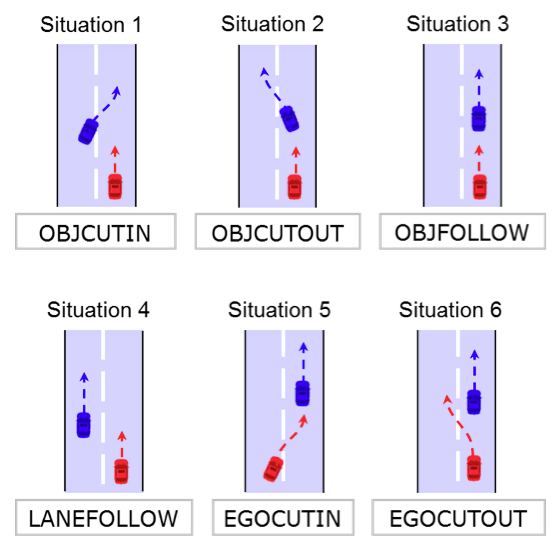
\includegraphics[scale=0.4]{./figures/DaimlerManeuvers}
\caption{\label{Figure:DaimlerManeuvers}Different maneuvers which should be identified by the AMIDST system.  Red blocks represents the EGO vehicle and blue blocks represents other vehicles in the scene. In the first four maneuvers, there is a lane change event or, under Daimler’s terminology, a ``Lane Marking Crossing'' (LMC) event. 
}
\end{center}
\end{figure}

The data used to address this problem do not contain raw data from the video, radar and on-board sensors. The early maneuver recognition system directly works with the so-called ``object data'', which contains ``high level'' representations or features describing the ``traffic scene'' such as EGO’s speed, distance between EGO and another vehicle in front, etc.  Figure \ref{Figure:DaimlerDataFlow} contains a visual description of the current data flow. 

\begin{figure}
\begin{center}
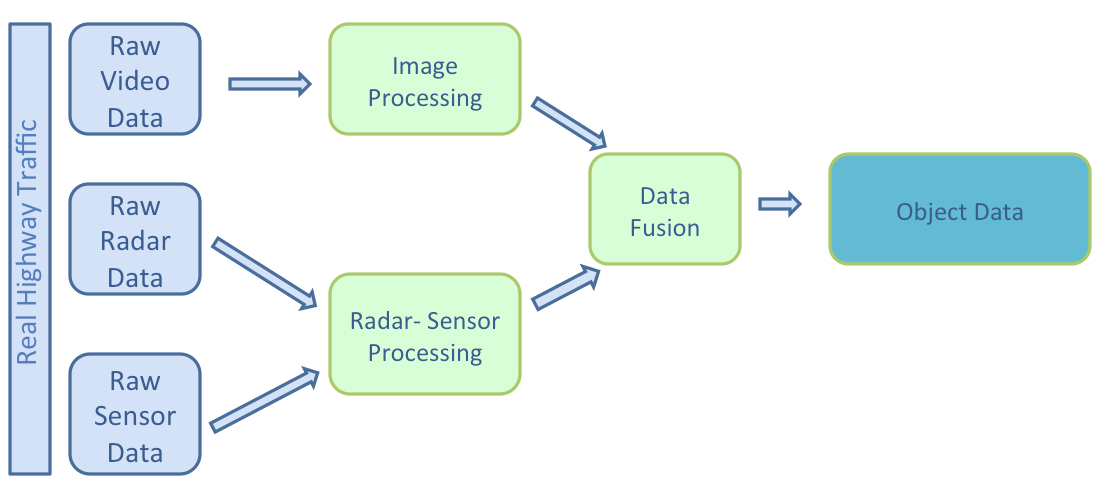
\includegraphics[scale=0.35]{./figures/DaimlerDataFlow}
\caption{\label{Figure:DaimlerDataFlow} Daimler's Data Flow.}
\end{center}
\end{figure}

As can be seen in the above figure, in a first step the raw data coming for the the video, radar and sensors is preprocessed. In a second step this preprocessed data is fused and the high-level or ``object data'' describing the traffic scene is obtained. 

Using this ``object data'', Daimler has developed a probabilistic graphical model [] which is able to recognize an ongoing maneuver around 0.6 seconds before the maneuver really takes place. This probabilistic approach is based on modelling the problem in different layers as shown in Figure \ref{Figure:DaimlerHierarchicalModelling}.
<<<<<<< HEAD
=======


\begin{figure}
\begin{center}
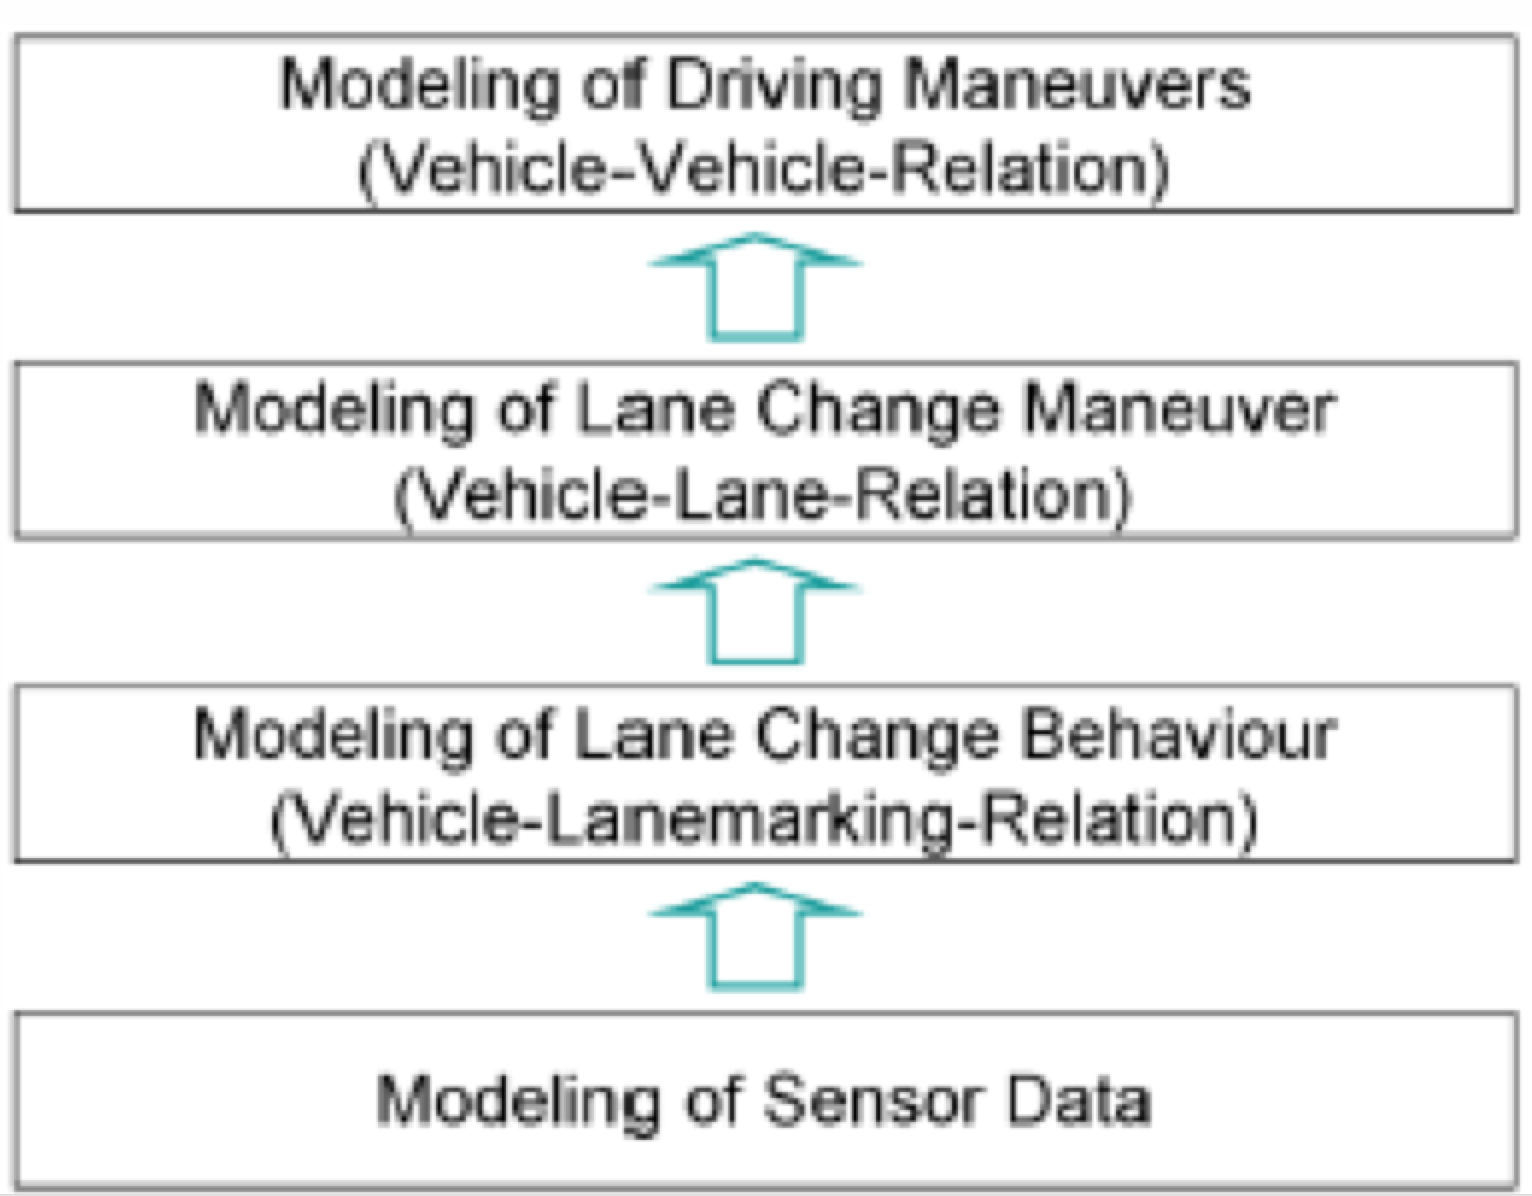
\includegraphics[scale=0.35]{./figures/DaimlerHierarchicalModelling}
\caption{\label{Figure:DaimlerHierarchicalModelling} Static-OOBN model for the prediction of an event (maneuver).}
\end{center}
\end{figure}

In a first step the sensor data is modelled and, sequentially,  a new layer is created on top of that to detect a lane change behaviour. Understanding the lane change behaviour of the vehicles, the system is able to model the lane change maneuver. And, with this information, the system is able to decide the kind of driving maneuver is taking place between pair of vehicles. 



\subsubsection*{The static-OOBN model}

As commented above, this model will work with ``object data''. This data mainly consists on a set of measured and/or computed signals or situation features denoted by $S$ (i.e. EGO speed, EGO lateral velocity, speed of a car in-front, etc.)  describing the traffic scene. 

The causal probabilistic treatment of these signals or situation features allows exploiting heterogeneous sources of information and the quantitative incorporation of uncertainties in the measured signals. The general structure of the static-OOBN model consists of a number of abstraction levels (see Figure \ref{Figure:DaimlerOOBNAbstraction}): all measured and/or computed signals $S$ are handled with their uncertainties $\sigma^2$. These are represented as object classes at the lowest level (class $S$) of the OOBN. The real values $\mu$ of evidence signals are then used at the next level of hierarchy to evaluate the hypotheses (class $H$ in Figure \ref{Figure:DaimlerOOBNAbstraction}). The combined evaluation of several hypotheses results in the prediction of events, class E. In our case: the events are modelling traffic maneuvers of the own and neighbour vehicles.

\begin{figure}
\begin{center}
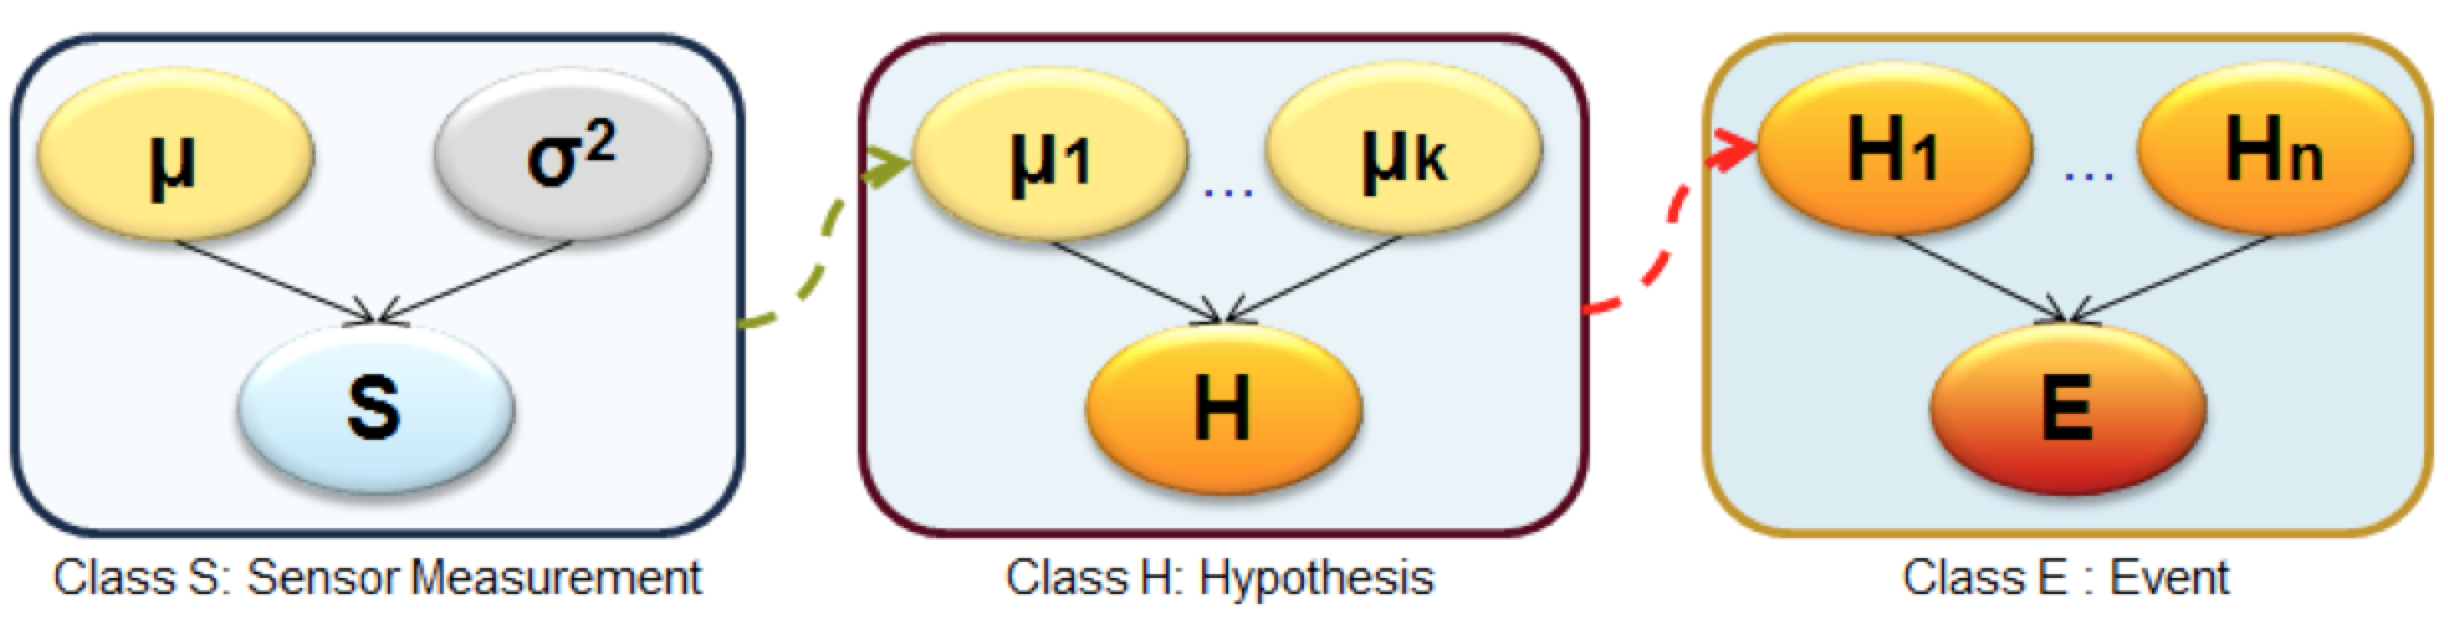
\includegraphics[scale=0.35]{./figures/DaimlerOOBNAbstraction}
\caption{\label{Figure:DaimlerOOBNAbstraction} Static-OOBN model for the prediction of an event (maneuver).}
\end{center}
\end{figure}

As commented above, the observations characterizing a situation are acquired from sensors and computations and, in consequence, are \textit{measured data}. If the measurement instrument is not functioning properly (due to sensor noise or fault), then the sensor-reading ($S\_MEASURED$) and the real variable ($S\_REAL$) under measurement need not to be the same. This fact imposes the causal model structure as shown in Figure \ref{Figure:DaimlerSensorModelling}. The sensor-reading of any measured variable is conditionally dependent on random changes in two variables: real value under measurement ($S\_REAL$) and sensor fault ($S\_SIGMA$).

\begin{figure}
\begin{center}
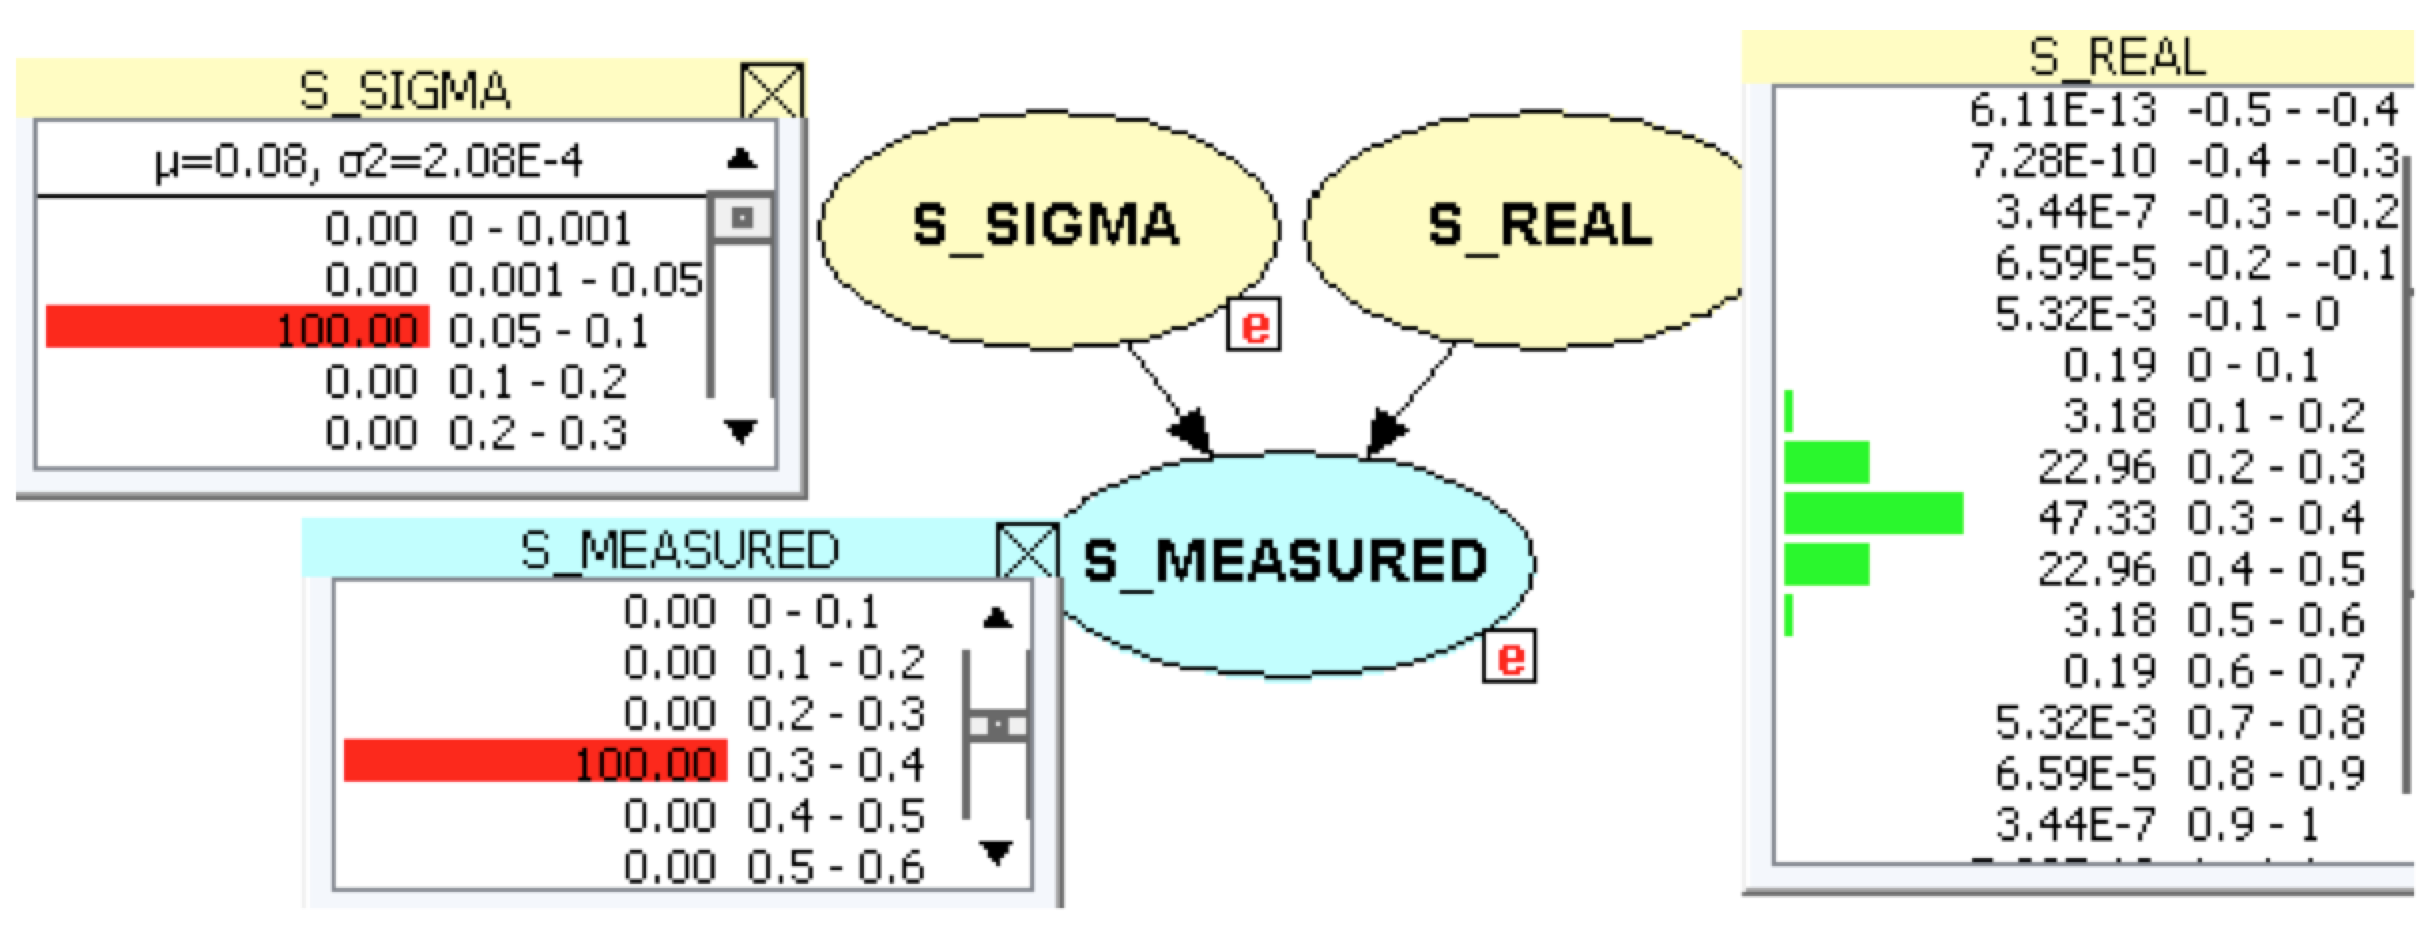
\includegraphics[scale=0.35]{./figures/DaimlerSensorModelling}
\caption{\label{Figure:DaimlerSensorModelling} BN fragment for modeling of sensor’s uncertainties with a discrete ``measurement'' variable.}
\end{center}
\end{figure}


The situation features used for maneuver recognition are structured along three main dimensions: lateral evidence (LE), trajectory (TRAJ), and occupancy schedule grid (OCCGRID). They represent the three hypotheses (see Figure \ref{Figure:DaimlerOOBNAbstraction}), which are modelled by the corresponding OOBN-fragments. For more details see [13], [14]. The hypothesis LE is shown in Figure \ref{Figure:DaimlerLE}. Its conditional probability distribution is represented by a sigmoid (logistic) function to expresses the growing probability for the lateral evidence on crossing the lane marking, when the vehicle is coming closer to the lane marking (modeled by $O\_LAT\_MEASURED$) by growing lateral velocity (modeled by $V\_LAT\_ MEASURED$).

\begin{figure}
\begin{center}
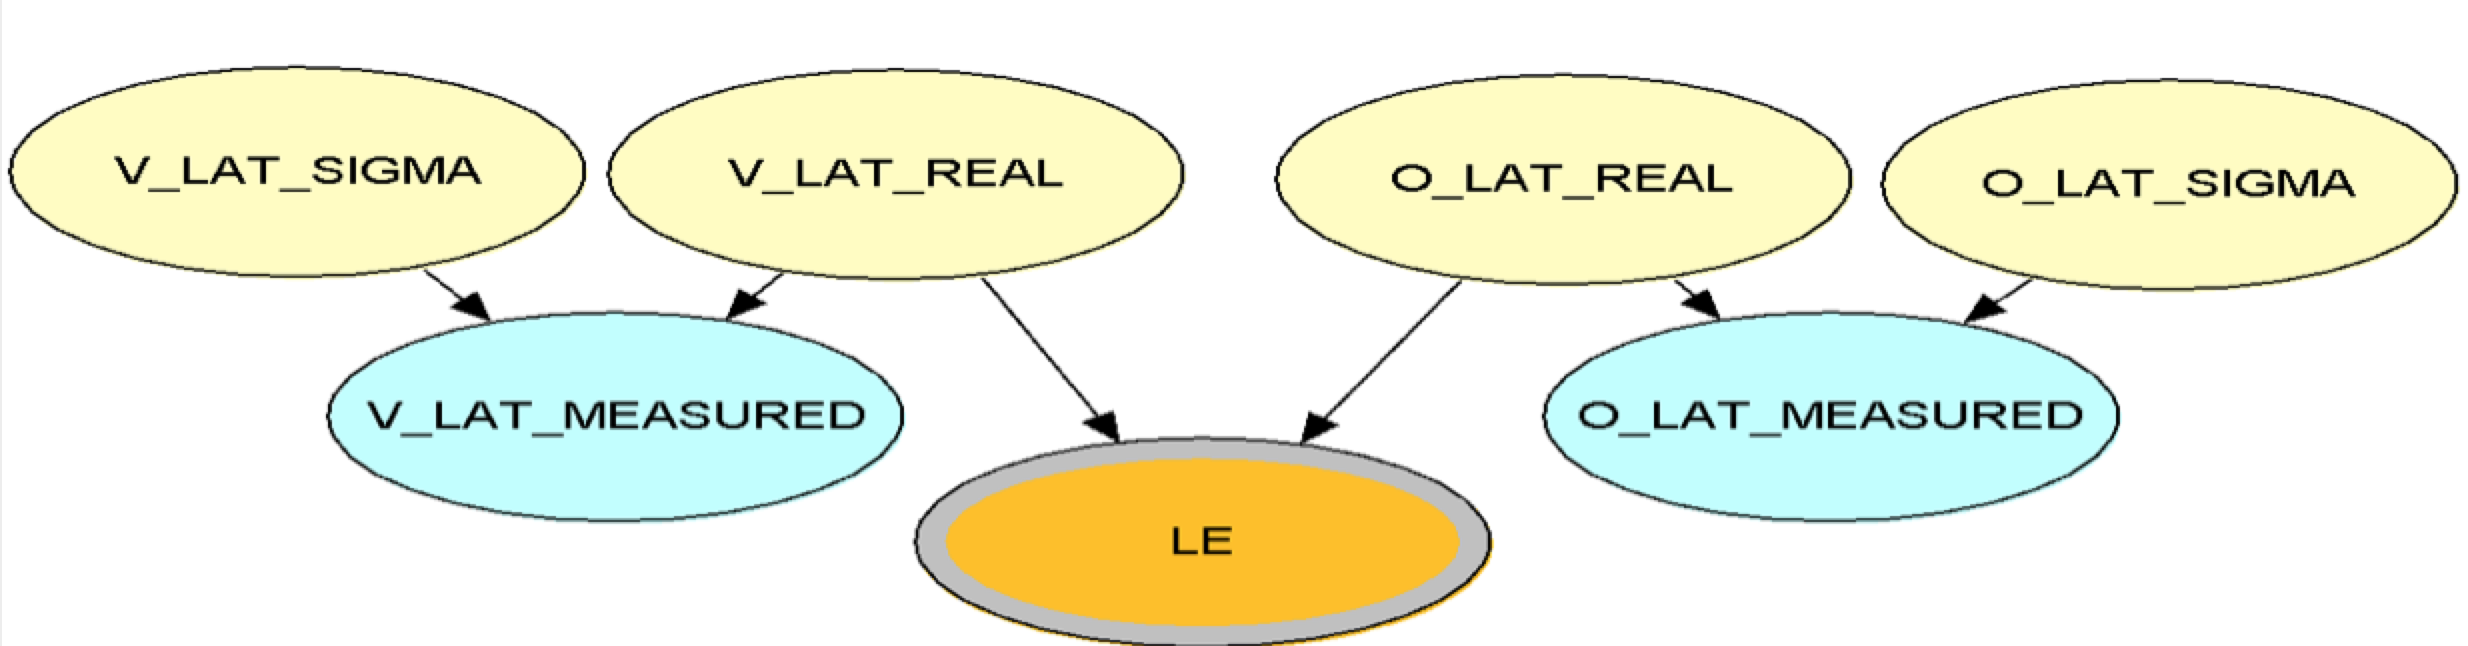
\includegraphics[scale=0.35]{./figures/DaimlerLE}
\caption{\label{Figure:DaimlerLE} BN fragment for modeling of sensor’s uncertainties with a discrete ``measurement'' variable.}
\end{center}
\end{figure}

Figure \ref{Figure:DaimlerOOBNAbstraction} abstractly shows how these hypotheses are combined into events, which in our automotive scenario correspond to the different driving maneuvers: lane follow, lane change (cut-in, cut-out), expressed for ego and surrounding objects, see [12], [13].

\subsubsection*{The dynamic-OOBN model}

The above described static OOBN is able to detect a maneuver 0.6s before execution. The goal is to extend the prediction horizon for manoeuvre recognition at least to 1-2 seconds (max. 4-5 seconds ahead) before the actual lane marking crossing, which is of advantage for the adaptive cruise control. Most precisely, and as indicated in the Use Case 8 on the Requirement Analysis,  the area under the ROC curve (AUC) should be greater than 0.96 for 1 second and greater than 0.9 for 2 seconds.

Figure [timedetection] shows the evolution on time for velocity and offset in an EGO\_CutOut manoeuvre. The vertical bar indicates the moment in which the manoeuvre has been recognised by the static OOBN. By taking the temporal properties of the data into account on the model, we should be able to predict the manoeuvre earlier on time.

Each manoeuvre can be considered as a process, developing in time, i.e., as data stream given by a time sequence of the transition from lane follow into lane change manoeuvre. The dynamic extension involves copies of the static OOBN for different number of time steps in the time window (e.g. see Fig. \ref{Figure:daimlerLEdyn} where the two top nodes are temporal clone defining the share belief state between consecutive time steps creating a first order Markov process), if also the requirement on earlier prognostics of maneuver is to be satisfied. 

\begin{figure}
\begin{center}
\caption{\label{Figure:daimlerLEdyn}Daimler Temporal Model}
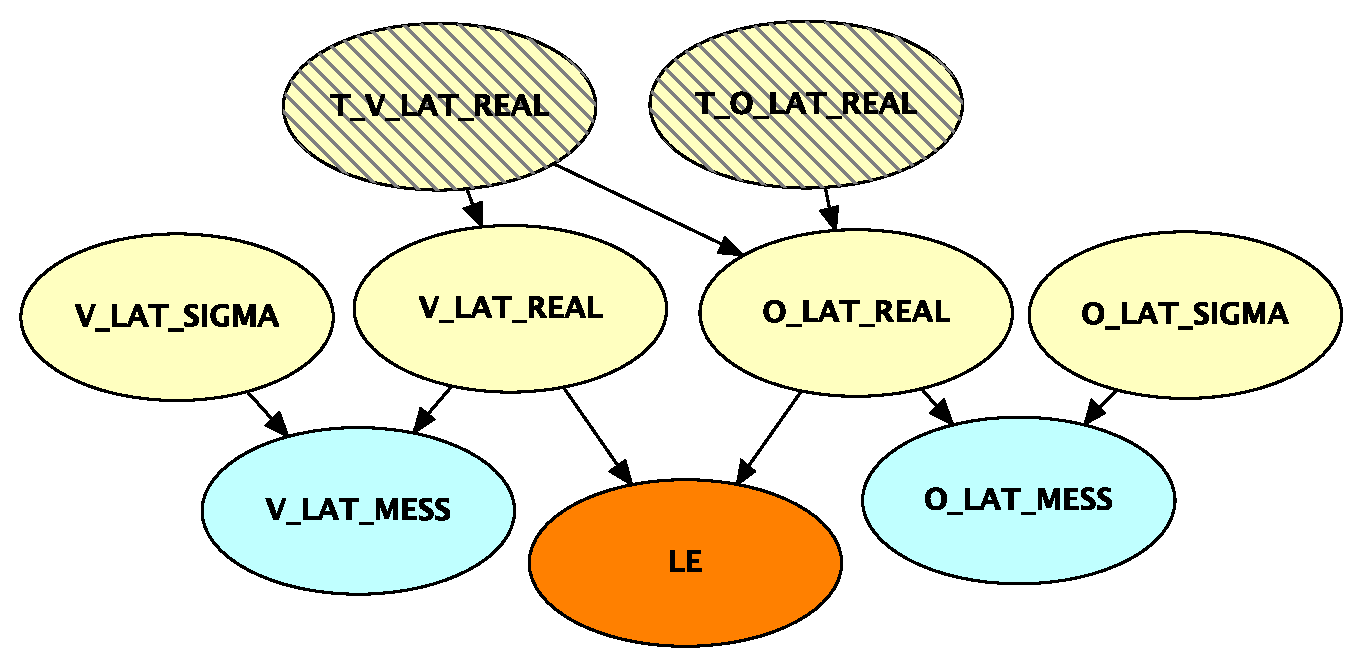
\includegraphics[scale=0.5]{./figures/LEdyn}
\end{center}
\end{figure}


\begin{enumerate}
\item \textbf{Dynamics on Lateral Evidence (LE)}
A good starting point to model the dynamics of the data involves the variables that capture the lateral evidence for the different vehicles, given its relevance and simplicity. 
The dynamic BN (DBN) incorporates the trend of change for the real values, where their physics relations are represented as causal dependencies between the time steps $dt$, e.g. in Fig. \ref{Figure:daimlerLEdyn} the transition function of O\_LAT at time $t$, O(t), is modeled as a Gaussian distribution. Its mean is affected by O(t-1), and by V\_LAT at time $t-1$, $v(t-1)$:

\begin{equation}
O(t) =O(t-1) +v(t-1)�dt +N
\end{equation}

where $N$ denotes a white noise $N(0,\sigma^2)$ due to possible acceleration term $(a�dt2)/2$, which is assumed to be small for a time step in the order of $102$ milliseconds.

The shaded nodes represent the development of the real values of observations over several time steps in the time window. Thus, their trend estimation contributes to the prediction of probability of transition from a lane follow to a lane change manoeuvre.

A DBN induces a number of constraints on the compilation of the network into a computational structure. One constraint relates to transferring the belief state from one time slice to the next where the belief state is the probability distribution over the variables shared by neighbouring time slices. In general, the belief state is transferred as a joint distribution. This means that approximate methods \cite{BoyenKoller} may have to be considered for meeting the requirements of the target platform.


\item \textbf{New hypothesis: Relative Dynamics (REL\_DYN)}

Earlier prediction of manoeuvre intentions can be achieved even before any development of the trend for lateral evidence LE has been observed. A first indication of possible lane change intention can be observed through the relative dynamics between one vehicle (host or object) and the vehicles in front of it on the same lane. Once again, the goal is to further increase the prediction horizon for manoeuvre recognition (up to 5 seconds). 

We can include qualitatively new information based on driving experience, which indicates a need for a lane change if a slower vehicle is driving in front of the own vehicle on the same lane. To continue its safe driving, the approaching vehicle should either break and reduce its speed to the speed of the vehicle in front or, alternatively,,it should change to the neighbour lane, if the neighbour lane is free and no other vehicle is approaching with a higher speed than the own vehicle. A continued safe manoeuvre (of type ``lane follow'' or ``lane change'') is modelled by estimating the TTC (TimeToCollision) to the vehicle in front (on the same lane) or to eventually approaching vehicle (on the neighbour lane). For safe manoeuvre, TTC should be bigger than 1 second, if the own vehicle wants to change to the neighbour lane or if it needs to break to ensure safe driving on the same lane (``'lane follow'') .

Figure [timedetectionRelDyn] shows the evolution on time for the velocity and distance in an EGO\_CutOut manoeuvre. The vertical bar indicates the moment in which the manoeuvre has been recognised by the static OOBN. By taking the temporal properties of the relative dynamics into account on the DBN, we should be able to predict the manoeuvre even earlier on time.

By analogy to Fig. \ref{Figure:daimlerLEdyn}, the original OOBN has been extended with the hypothesis ``relative dynamics'' (REL\_DYN), as shown in Fig.\ref{Figure:daimlerreldyn}. This BN fragment  models the hypothesis REL\_DYN with 3 states Left/Follow/RIGHT, utilising the independency assumption for the discrete variables V\_REL\_MEASSURED and X\_REL\_MEASSURED.

\begin{figure}
\begin{center}
\caption{\label{Figure:daimlerreldyn}Daimler Temporal Model with relative dynamics}
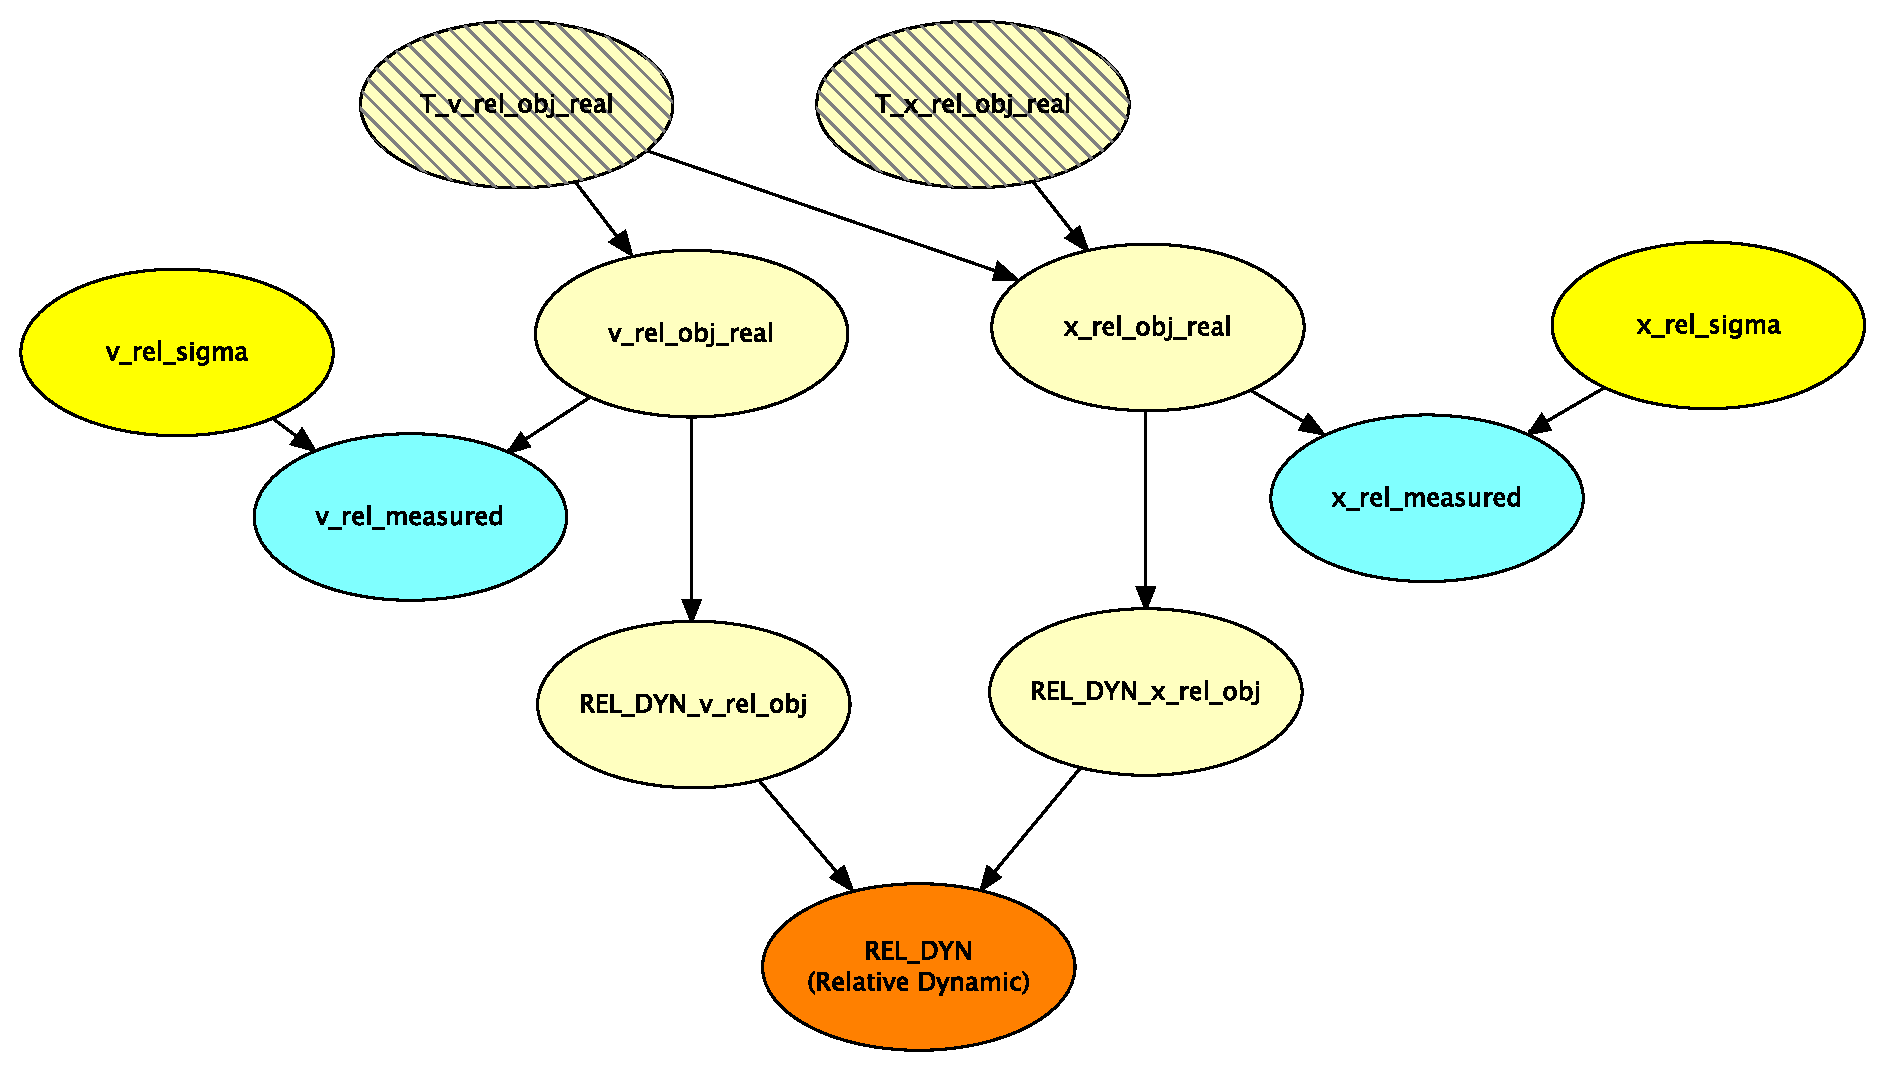
\includegraphics[scale=0.4]{./figures/reldyn}
\end{center}
\end{figure}

If we compare the structure of this network with that of Fig. \ref{Figure:daimlerLEdyn}, we can observe two additional nodes:  REL\_DYN\_V\_REL\_OBJ and REL\_DYN\_X\_REL\_OBJ. They are the results of a modelling trick to simplify the EM-learning of parameters from data for the static BN fragment.

\textcolor{red}{Note that the new REL\_DYN hypothesis introduced would require two instances in the OOBN, one for the relative dynamics of the EGO with the OBJ in front, and another one for the OBJ and another OBJ in front of it. Each REL\_DYN would indicate if the EGO and the OBJ cars are going to turn right, left or continue straight.}

\end{enumerate}
